%%%%%%%%%%%%%%%%%%%%%%%%%%%%%%%%%%%%%%%%%%%%%%%%%%%%%%%%%%%%%%%%%%%%%%%%%%%%%%%%%%%%%%%%%%%%%%%%%%%

%% document class
%\documentclass{beamer}
%\documentclass[aspectratio=169]{beamer}
\documentclass[handout]{beamer}

%% packages
\usepackage{multimedia}
%% packages


\usepackage{braket}%braketnotationpackage


%% page settings
%% Theme
\usetheme{Berkeley} % theme for slides
%\usetheme{Frankfurt}
%\usetheme{Madrid}

%% Colors
%\usecolortheme{rose} % color for slides
\usecolortheme{beetle}
\definecolor{c1}{rgb}{0.5,0.5,0.5} % some green
\definecolor{c2}{rgb}{0.2,0.9,0.1} % some gray
%% see http://www.sharelatex.com/learn/Beamer
%\setbeamercolor*{palette primary}{fg=white,bg=c1} % upper part
%\setbeamercolor*{palette secondary}{bg=c2} % left part (background)
%\setbeamercolor*{sidebar left}{fg=white,bg=c1} % left part with links
%\setbeamerfont{section number projected}{ % section numbers
%  family=\rmfamily,
%  series=\bfseries,
%  size=\normalsize
%  }
%\setbeamercolor{section number projected}{bg=c1} % color of section numbers and others (fg: Fontm, bg:Hintergrund)
%\setbeamercolor{item projected}{bg=c1}
%\setbeamercolor{itemize item}{fg=c1}
%\setbeamercolor{author in sidebar}{fg=white}
%\setbeamercolor{footlinecolor}{fg=black,bg=c2}

%% Fonts
\usefonttheme{professionalfonts} % changes fonts

%% Foot
\usenavigationsymbolstemplate{} % deafult controls off
\setbeamertemplate{footline}[frame number] % slide number at the bottom
%\setbeamertemplate{footline}
%{%
%	\leavevmode%
%	\hbox{%
%	\begin{beamercolorbox}[wd=.3\paperwidth,ht=5ex,dp=1.5ex,left,leftskip=2mm]{footlinecolor}%
%		Foot information on the left over several lines
%	\end{beamercolorbox}%
%	\begin{beamercolorbox}[wd=.5\paperwidth,ht=5ex,dp=1.5ex,left,leftskip=2mm]{footlinecolor}%
%		Next foot part
%	\end{beamercolorbox}%
%	\begin{beamercolorbox}[wd=.2\paperwidth,ht=5ex,dp=1.5ex,right,rightskip=2mm]{footlinecolor}%
%		\insertframenumber{} / \inserttotalframenumber%
%	\end{beamercolorbox}%
%	}%
%	\vskip0pt%
%}

%% new commands
\newcommand{\cm}[1]{{\tt \textcolor{orange}{#1}}}
\newcommand{\wl}[2]{\href{#2}{\textcolor{blue}{#1}}}
\newcommand{\att}[2]{\href{#2}{\textcolor{blue}{#1}}}

%%%%%%%%%%%%%%%%%%%%%%%%%%%%%%%%%%%%%%%%%%%%%%%%%%%%%%%%%%%%%%%%%%%%%%%%%%%%%%%%%%%%%%%%%%%%%%%%%%%

\begin{document}

\author[Stefanopoulos]{Stefanopoulos Dimitrios}
\title[Quantum Thermodynamics]{Statistical Mechanics from Quantum Thermodynamics}
\titlegraphic{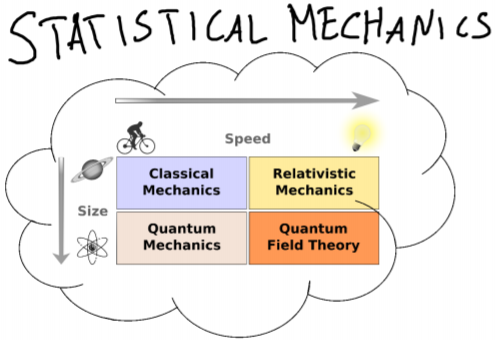
\includegraphics[width=0.3\textwidth]{figures/heat}}
\institute{Aristotle's University of Thessaloniki}
\date{Thessaloniki, \today}
\frame{\titlepage}

%%%%%%%%%%%%%%%%%%%%%%%%%%%%%%%%%%%%%%%%%%%%%%%%%%%%%%%%%%%%%%%%%%%%%%%%%%%%%%%%%%%%%%%%%%%%%%%%%%%

\begin{frame}{Table of contents}
\tableofcontents
%\tableofcontents[hideallsubsections]
\end{frame}

%%%%%%%%%%%%%%%%%%%%%%%%%%%%%%%%%%%%%%%%%%%%%%%%%%%%%%%%%%%%%%%%%%%%%%%%%%%%%%%%%%%%%%%%%%%%%%%%%%%
%%%%%%%%%%%%%%%%%%%%%%%%%%%%%%%%%%%%%%%%%%%%%%%%%%%%%%%%%%%%%%%%%%%%%%%%%%%%%%%%%%%%%%%%%%%%%%%%%%%

\section{Intro}
\subsection{Motivations}
\begin{frame}{Need for quantum foundations of statistical mechanics}
\begin{itemize}
\item Quantum probability amplitudes are not consistent with the axiom of a priori equal probability(at least not on first sight)
\item Absence of unitarity in the evolution of thermodynamic systems
\item Further applications
\end{itemize}
\end{frame}
\subsection{Density Matrix Formalism}
\begin{frame}{Density Matrix}
\begin{itemize}
\item The definition:
\begin{equation}
\rho=\sum_{j} p_{j}\left|\psi_{j}\right\rangle\left\langle\psi_{j}\right|
\end{equation}
\item Quantum Randomness vs Classical Randomness:
\begin{equation}\sum p_j =1
\end{equation}
\item The canonical state:
\begin{equation}
\Omega_{S}=(1-p)^{k} \sum_{s} \exp \left(-\frac{|s| B}{\mathrm{k}_{B} T}\right)|s\rangle\langle s|
\propto \exp \left(-\frac{H_{S}}{\mathrm{k}_{B} T}\right)
\label{Omega}
\end{equation}
\end{itemize}

\end{frame}
\subsection{Assumptions}
\begin{frame}{Assumptions}
\begin{itemize}
\item Restricted Subspace $R$
\begin{equation}\mathcal{H}_{R} \subseteq \mathcal{H}_{S} \otimes \mathcal{H}_{E}
\end{equation}
\begin{center}
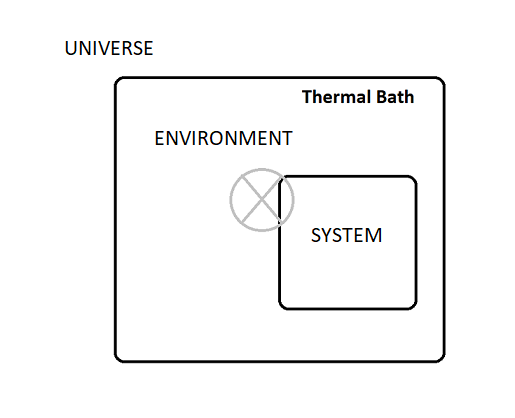
\includegraphics[scale=0.4]{figures/photo}
\end{center}

\item Equiprobable:
\begin{equation}
\mathcal{E}_{R}=\frac{\mathbb{I}_{R}}{d_{R}}
\label{equiprob}
\end{equation}
\item State of the system:
\begin{equation}\Omega_{S}=\operatorname{Tr}_{E}\left(\mathcal{E}_{R}\right)
\end{equation}
\end{itemize}
\end{frame}
%%%%%%%%%%%%%%%%%%%%%%%%%%%%%%%%%%%%%%%%%%%%%%%%%%%%%%%%%%%%%%%%%%%%%%%%%%%%%%%%%%%%%%%%%%%%%%%%%%%

\section{Theories}
\subsection{Typicality}
\begin{frame}{Typicality}
\begin{itemize}
\item We compare with a pure state of the Universe:
\item Typicality is a naturally statistical equality of an observable in the two cases (i.e. pure or maximally mixed state of the universe)
\begin{equation}
\rho_{S}= \operatorname{Tr}_{E}(\ket{\psi}\bra{\psi})
\end{equation}
\item It has been proven that for sufficiently large 
dimensions of the environment(i.e. possible states):
\begin{equation}
||\rho_S-\Omega_S||\approx 0
\end{equation}

\end{itemize}

\end{frame}
\subsection{Environment assisted invariance}
\subsubsection{Definition}
\begin{frame}{Envariance}
\begin{itemize}
\item There are arguments that the symmetry of envariance can produce Born's rule and Thermal States.
\item \ $\psi_{SE}$ is called envariant under a unitary map $U_{\mathcal{S}}=u_{S} \otimes \mathbb{I}_{E}$ iff there exists another unitary $U_{E}= \mathbb{I}_{E} \otimes u_{E} $ such that:
\begin{equation}
\begin{array}{l}
U_{S}\left|\psi_{S E}\right\rangle=\left(u_{S} \otimes \mathbb{I}_{E}\right)\left|\psi_{S E}\right\rangle=\left|\eta_{S E}\right\rangle \\
U_{E}\left|\eta_{S \mathcal{E}}\right\rangle=\left(\mathbb{I}_{S} \otimes u_{E}\right)\left|\eta_{S E}\right\rangle=\left|\psi_{S E}\right\rangle
\end{array}
\end{equation}
\end{itemize}
\end{frame}
\subsubsection{Demonstration}

\begin{frame}{Envariance}
To illustrate the above we state a simple example. Let $\mathcal{S}$ and $E$ be two level systems and assume that $\left|\psi_{SE}\right\rangle \propto|\uparrow\rangle_{S} \otimes|\uparrow\rangle_{E}+|\downarrow\rangle_{S} \otimes|\downarrow\rangle_{E}$. 
\begin{equation}
|\uparrow\rangle_{\mathcal{S}} \otimes|\uparrow\rangle_{E}+|\downarrow\rangle_{\mathcal{S}} \otimes|\downarrow\rangle_{E} \stackrel{U_{\mathcal{S}}}{\longrightarrow}|\downarrow\rangle_{\mathcal{S}} \otimes|\uparrow\rangle_{E}+|\uparrow\rangle_{\mathcal{S}} \otimes|\downarrow\rangle_{E}
\end{equation}
\begin{equation}
|\downarrow\rangle_{\mathcal{S}} \otimes|\uparrow\rangle_{E}+|\uparrow\rangle_{\mathcal{S}} \otimes|\downarrow\rangle_{E} \stackrel{U_{E}}{\longrightarrow}|\downarrow\rangle_{\mathcal{S}} \otimes|\downarrow\rangle_{E}+|\uparrow\rangle_{\mathcal{S}} \otimes|\uparrow\rangle_{E}
\end{equation}
\end{frame}
\section{Conclusions}
\begin{frame}{Conclusions}
\begin{itemize}
\item Quantum Thermodynamics promises a lot about the foundations of Statistical Mechanics
\item Information Theoretic Approaches are quite convincing and the are obviously have something to do with Statistical Mechanics in general.
\item Quantum Entanglement is of a vital importance in the production of Statistical Mechanics Formulas via Hilbert Spaces.
\end{itemize}
\end{frame}
\begin{frame}{The end}
\begin{center}
\Huge Thank you!!!!
\end{center}
\end{frame}
\end{document}
